\documentclass[conf]{new-aiaa}
%\documentclass[journal]{new-aiaa} for journal papers
\usepackage[utf8]{inputenc}

\usepackage{graphicx}
\usepackage{amsmath}
\usepackage[version=4]{mhchem}
\usepackage{siunitx}
\usepackage{longtable,tabularx}
\usepackage{footnote}
\usepackage{mhchem}
\makesavenoteenv{tabular}
\setlength\LTleft{0pt} 

\title{Preparation of Papers for AIAA Technical Conferences}

\author{First A. Author\footnote{Insert Job Title, Department Name, Address/Mail Stop, and AIAA Member Grade (if any) for first author.} and Second B. Author Jr.\footnote{Insert Job Title, Department Name, Address/Mail Stop, and AIAA Member Grade (if any) for second author.}}
\affil{Business or Academic Affiliation 1, City, State, Zip Code}
\author{Third C. Author\footnote{Insert Job Title, Department Name, Address/Mail Stop, and AIAA Member Grade (if any) for third author.}}
\affil{Business or Academic Affiliation 2, City, Province, Zip Code, Country}
\author{Fourth D. Author\footnote{Insert Job Title, Department Name, Address/Mail Stop, and AIAA Member Grade (if any) for fourth author (etc.).}}
\affil{Business or Academic Affiliation 2, City, State, Zip Code}

\begin{document}

\maketitle

\begin{abstract}
These instructions give you guidelines for preparing papers for AIAA Technical Papers using \LaTeX{}. Define all symbols used in the abstract. Do not cite references in the abstract. The footnote on the first page should list the Job Title and AIAA Member Grade for each author, if known Authors do not have to be AIAA members.
\end{abstract}

\section{intro/motivation}

\section{Description of Recovery Strategies}
Although only two vehicles with recoverable stages have been operated, a wide variety of first stage recovery strategies have been proposed. This section seeks to develop a systematic classification of recovery strategies, which will be useful in comparing their relative merits.

First stage recovery strategies can be characterized by three high-level choices:
\begin{enumerate}
	\item \textit{Portion of stage recovered} - Some strategies recover the entire first stage, while others propose to only recover a portion containing the higher-value components (e.g. main engines).
	\item \textit{Deceleration and maneuvering method} - The first stage must have some means to control and slow its re-entry trajectory. The deceleration and maneuvering methods can be grouped into three categories: propulsive designs which use the main engines to maneuver and land vertically; winged designs which use aerodynamic surfaces to maneuver and land horizontally; and design which decelerate using parachutes. Note that these are not absolute distinctions: current propulsive-landing designs use small aerodynamic control surfaces, and some proposed winged designs have auxiliary propulsion to increase their range.
	\item \textit{Recovery location} - The stage may be recovered downrange, or may fly itself back for recovery launch site. Most downrange recovery strategies land on a boat or in the ocean, although some call for the recovered components to be caught by an aircraft in midair \cite{Ragab2015}.
\end{enumerate}

Figure \ref{fig:recov_strat_diagram} illustrates the concept of operations for various strategies formed from the above choices. Strategies which have been carried out or proposed are listed in Table \ref{tab:vehicles}, and along the bottom of Figure \ref{fig:recov_strat_diagram}.

\begin{figure}[hbt!]
	\centering
	\includegraphics[width=1\textwidth]{figures/recov_strat_diagram}
	\label{fig:recov_strat_diagram}
	\caption{Recovery strategies TODO better graphics}
\end{figure}

\begin{table}
	\caption{\label{tab:vehicles} Some launch vehicles with reusable first stages. (* denotes boosters used in parallel staging)}
	\centering
	\begin{tabular}{p{4cm} l p{2cm}  p{2cm} p{2cm}}
		\hline
		Vehicle & Status & Portion of booster recovered & Deccel \& Manuever method & Recovery location \\
		\hline
		\hline
		Falcon 9 & Operational & Full & Propulsive & Launch site or downrange \\
		\hline
		Space Shuttle* & Retired & Full & Parachute & Downrange \\
		\hline
		New Glenn & Proposed & Full & Propulsive & Downrange \\
		Adeline (Ariane 6) & Proposed & Partial & Wing & Launch site \\
		SMART (Vulcan) \cite{Ragab2015} & Proposed & Partial & Parachute & Downrange midair \\
		\hline
		Ares I \cite{Ares2009} & Canceled & Full & Parachute & Downrange \\
		Reusable Booster System (RBS) \cite{NAP13534} & Canceled & Full & Propulsive \& Wing & Launch site\\
		NASA Liquid Fly-Back Booster (LFBB)* \cite{Healy1998} & Canceled & Full & Propulsive \& Wing & Launch site\\
		DRL Liquid Fly-Back Booster (LFBB)* \cite{Sippel2003} & Canceled & Full & Propulsive \& Wing & Launch site\\
		\hline
	\end{tabular}
\end{table}

Despite their wide variety, all these strategies face the same fundamental tradeoff between performance and cost. On the performance side, all recovery strategies require the first stage to carry extra mass during ascent, reducing the payload which can be lifted to orbit. However, recovering and reusing some of the first stage has the potential to reduce launch costs by eliminating the need to re-build expensive hardware\footnote{A reduction in cost is by no means guaranteed. As the Space Shuttle program demonstrated, excessive refurbishment and operations costs can make a reusable system more expensive than expendable alternatives.}. We should expect that recovery strategies will differ in their performance penalty and potential for cost reduction. The fundamental question is which, if any, of the recovery strategies can offer a small enough payload reduction and a large enough cost reduction to be worthwhile?

To make this question more concrete, this paper defines two figures of merit for recovery strategies: the payload factor $r_p$ and the cost factor $r_c$. These factors compare the payload capacity and cost of a vehicle with a reusable first stage to an equivalent\footnote{The `equivalent' expendable vehicle uses the same propulsion and structural technologies, and has the same gross liftoff mass $m_{0,1}$} vehicle with an expendable first stage. The payload factor is the payload capacity of the partially reusable vehicle divided by the payload capacity of the equivalent expendable vehicle. The cost factor is the average flight cost of the reusable first stage divided by the average flight cost of an expendable first stage.

When comparing recovery strategies, we can largely neglect their internal complexities and consider each strategy to be represented by a tuple $\mathcal{R}: \{r_p, r_c\}$. We seek recovery strategies with high payload factor ($r_p \rightarrow 1$) and low cost factor ($r_c \rightarrow 0$).

The following two sections attempt to provide quantitative, first-principles tools to estimate $r_p$ and $r_c$. The payload factor can be easily estimated with a fair degree of accuacy, but cost modeling involves more guesswork. The TODO nth section examines the trade-offs between different strategies. Because the willingness of a launch provider to trade payload for cost is uncertain, this comparison is framed to yield a set of recovery strategies which is Pareto-optimal in $(r_p, r_c)$.




\section{Performance Model}
TODO
This section provides a general, first-principles framework for estimating the payload reduction factor $r_p$ of a recovery strategy. The fundamental cause of payload reduction is that a recoverable stage must carry extra mass, as recovery hardware or propellant reserved for recovery maneuvers. This extra mass reduces the fraction of the stage's mass which is expelled during ascent. To still deliver the required $\Delta v$ to the payload, the payload mass fraction must then be reduced.

\subsection{Payload factor and first stage unavailable mass}
This subsection establishes a relationship between the payload factor $r_p$ and the extra mass carried on the first stage for recovery.
The reduction in payload can be seen from the Tsiolkovsky rocket equation. For a two-stage, sequentially stage rocket, the equation is \cite{Wiesel2010}:

\begin{equation}
\Delta v_* =  \sum_{i=1}^{2} - c_i \ln\left( \epsilon_i + (1 - \epsilon_i) \pi_i \right)
\end{equation} 

$\Delta v_*$ is the `mission $\Delta v$' required to lift the payload to its desired orbit. $c_i$ is the effective exhaust velocity ($c = I_{sp} g_0$) of stage $i$, averaged over the ambient pressures at which the stage operates. The log-mass term is written in terms of the dimensionless parameters $\epsilon_i$ and $\pi_i$. $\epsilon_i$ is the inert mass fraction of stage $i$; it depends only on the design of the stage.

\begin{equation}
\epsilon_i = \frac{m_{s,i}}{m_{s,i} + m_{p,i}}
\end{equation}

$\pi_i$ is the mass of the stage's payload (including all higher stages) divided by the gross mass at stage ignition:

\begin{equation}
\pi_1 = \frac{m_{0,2}}{m_{0,1}}, \quad \pi_2 = \frac{m_*}{m_{0,2}}
\end{equation}

The overall payload ratio of the launch vehicle, $\pi_*$ is the product of the stage payload ratios:

\begin{equation}
\label{eq:pi_star}
\pi_* = \frac{m_*}{m_{0,1}} = \pi_1 \pi_2
\end{equation} 

Modifying the rocket for first stage recovery effectively increases the inert mass fraction of the first stage to some new value $\epsilon_1'$. I will call $\epsilon_1'$ the `unavailable mass fraction', as it is the fraction of the first stage's mass which is unavailable for expulsion to propel the ascent. It includes the mass of the first stage structure ($m_{s,1}$) , the mass of recovery hardware ($m_{rh,1}$), and the mass of propellant reserved for recovery maneuvers ($m_{pr,1}$). The unavailable mass fraction can also be thought of as the first stage mass at stage separation divided by the first stage mass at liftoff.

\begin{equation}
\epsilon_1' = \frac{m_{s,1} + m_{rh,1} + m_{pr,1}}{m_{s,1} + m_{rh,1} + m_{p,1}}
\end{equation}

Then, the rocket equation for ascent is
\begin{equation}
\label{eq:recov_rocket}
\Delta v_* =  - c_1 \ln\left( \epsilon_1' + (1 - \epsilon_1') \pi_1 \right) - c_2 \ln\left( \epsilon_2 + (1 - \epsilon_2) \pi_2 \right)
\end{equation}

Our goal is to use Equation \ref{eq:recov_rocket} to determine how changes to $\epsilon_1'$ affect $\pi_*$. To do this, we need to introduce a few additional constraints. First, we assume that the stage 2 / stage 1 mass ratio has a some value $y$.

\begin{equation}
y = \frac{m_{s,2} + m_{p,2}}{m_{s,1} + m_{rh,1} + m_{p,1}}
\end{equation}

It can be shown that

\begin{equation}
\label{eq:ypi}
\pi_2 = (y + 1) - \frac{y}{\pi_1}
\end{equation}

Second, we define a `technology choice', $\mathcal{T}$, which influences the mass ratios and exhaust velocities. This choice encompasses technological factors such as the propellant (e.g. \ce{O2(l)}/kerosene vs. \ce{O2(l)}/\ce{H2(l)}), the tank construction technology (e.g. aluminum alloy vs. composite), and the engine cycle (e.g. gas generator vs. staged combustion). For the purposes of this model, the technology choice is fully described by the tuple $\mathcal{T} : \{ c_1, c_2, E_1, E_2 \}$, where $E$ is the technological lower limit on the structural mass fraction of an expendable stage. For expendable stages, $\epsilon_i = E_i$. For recoverable stages, $\epsilon_1' > E_1$.

If we know $\Delta v_*$ (set by the mission), the technology choice $\mathcal{T}$, and the stage mass ratio $y$, we can find $\pi_*(\epsilon_1`)$ from Equations \ref{eq:pi_star}, \ref{eq:recov_rocket}, and \ref{eq:ypi}. Then, we can compare the payload capacity of the recoverable rocket to that of an equivalent expendable rocket to find the payload factor $r_p$. First, we will make our definition of `equivalent expendable rocket' more rigorous: the `equivalent' rocket uses the same technology choice, the same stage mass ratio, and has the same gross liftoff mass. We also assume that the mission $\Delta v_*$ is the same for both rockets \footnote{We might expect this assumption to be incorrect if the recovery strategy changes the $\Delta v$ losses during ascent (e.g. increased drag due to wings). However, an analysis by DRL finds that ``The impact of the different RLV-types [reusable launch vehicle] on the ascent flight profile is found small and, similar to the ELV [expendable launch vehicle] ascent flight performance losses, these are more dependent on the particular configuration with its T/W [thrust to weight] ratio than on the landing and return modes.'' \cite{Stappert2017}.}

\begin{equation}
\mathcal{T}^{\mathrm{expend}} = \mathcal{T}^{\mathrm{recov}}, \quad y^{\mathrm{expend}} = y^{\mathrm{recov}}, \quad m_{0,1}^{\mathrm{expend}} = m_{0,1}^{\mathrm{recov}}, \quad \Delta v_*^{\mathrm{expend}} = \Delta v_*^{\mathrm{recov}}
\end{equation}

Finally, the payload factor is

\begin{equation}
r_p = \frac{m_*^{\mathrm{recov}}}{m_*^{\mathrm{expend}}} = \frac{\pi_*^{\mathrm{recov}}}{\pi_*^{\mathrm{expend}}}
\end{equation}

The relation of $r_p$ to $\epsilon_1`$ is shown in Figure \ref{fig:payload} two typical launch missions (Low Earth Orbit $\Delta v_* = \SI{9.5}{\kilo\meter\per\second}$ and Geostationary Transfer Orbit $\Delta v_* = \SI{12.0}{\kilo\meter\per\second}$). As expected, the payload capacity declines with increasing first stage unavailable mass. Also, note that the decline is more severe for higher $\Delta v_*$ missions. Thus, a particular recovery strategy (with some $\epsilon_1'$) will have a smaller payload factor for GTO missions than for LEO missions ($r_p^{\mathrm{LEO}} > r_p^\mathrm{GTO}$). Higher $\Delta v_*$ missions put a bigger penalty on first stage recovery. 

\begin{figure}[hbt!]
	\centering
	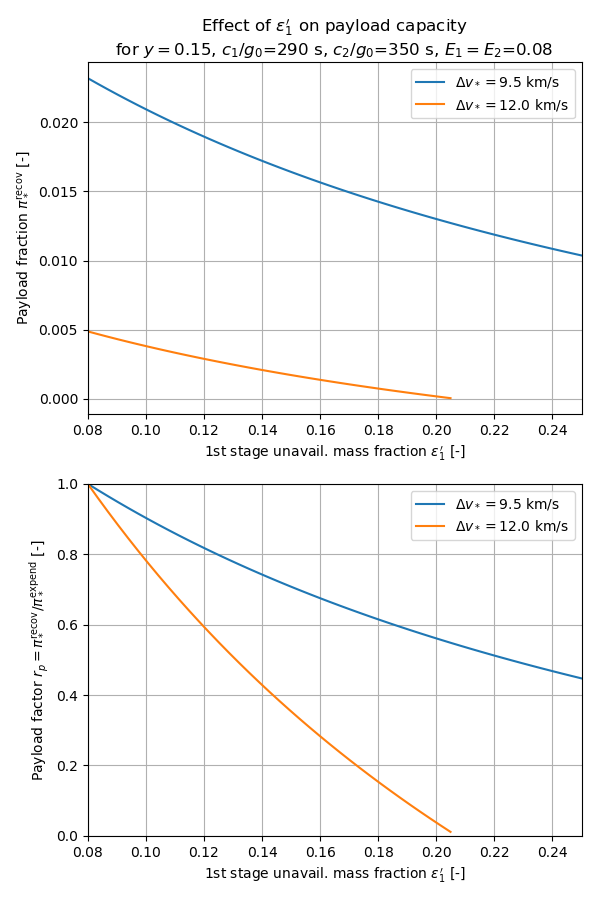
\includegraphics[width=0.5\textwidth]{../payload}
	\label{fig:payload}
	\caption{Impact of first stage unavailable mass fraction $\epsilon_1'$ on payload capability. Note that the payload factor $r_p$ declines with increasing unavailable mass, and the decline is more severe for higher $\Delta v_*$ missions. The technology choice values are typical for \ce{O2(l)}/kerosene and aluminum tanks.}
\end{figure}


\subsection{Determining the unavailable mass from recovery hardware and maneuvers}





\section{Cost Model}
Next, we attempt to quantify the cost savings from reusing the first stage. The cost savings are quantified by the cost factor $r_c$, which is the ratio of the average cost of one flight of a reusable first stage to the average cost of an expendable first stage. For $r_c < 1$, the reusable system has lower recurring costs. Write $r_c$ in terms of some of the cost elements identified in \cite{Sforza2015}:

\begin{equation}
\label{eq:cost_elements}
r_c = \frac{\frac{C_{pr}}{n} + C_{pn} + C_f + C_{ro}}{C_{pe}}
\end{equation}

where $n$ is the average lifetime number of flights for a reusable first stage. The cost elements of the reusable first stage are: $C_{pr}$, the production cost of the reusable components; $C_{pn}$, the production cost of the new (non-reusable) components; $C_f$, the refurbishment cost; and $C_{ro}$, the recovery operations cost. The expendable stage production cost is $C_{pe}$. Note that this cost model does not capture development costs. Also, $r_c$ only includes those costs directly relevant to the first stage, and excludes other factors which contribute to the launch service cost (upper stage, facilities, and insurance, etc.).

Actual costs vary with booster size scale, are difficult to estimate for new vehicle proposals \cite{Sforza2015}, and are often not publicly available. Instead, it is more helpful to write the cost factor in terms of dimensionless ratios which can be more readily estimated. I define the following ratios:
\begin{itemize}
	\item The recovered cost ratio, $z$, which is the ratio of the cost of the recovered hardware to the total production cost of the recoverable stage
    \begin{equation}
    z = \frac{C_{pr}}{C_{pr} + C_{pn}}
    \end{equation}
    By definition, $z \in [0, 1]$. For full-recovery strategies, $z=1$. For strategies which recover only the engines and other high-value components, $z \approx 0.5$ \cite{Ragab2015} (TODO more general engine cost as fraction of stage cost. I think Atlas V has a unusually expensive engine).
    
    \item The recovery and refurbishment cost ratio, $q$, which is the cost of recovery and refurbishment divided by production cost of the reusable hardware.
    \begin{equation}
    q = \frac{C_{f} + C_{ro}}{C_{pr}}
    \end{equation}
    By definition, $q > 0$. Inefficient recovery strategies can have $q > 1$ (e.g. SRB citation needed), in which case recovery cannot lead to cost savings and is probably not worthwhile. In some extreme proposals, the only recovery/refurbishment operation would be to reload the stage with propellant \cite{Musk2017}. In this case, propellant costs give a lower limit of $q \approx 0.01$ for hydrocarbon/oxygen stages \cite{Ragab2015}. A more moderate estimate from \cite{Sforza2015} gives $q \approx 0.25$ (15\% for refurbishment and another 10\% for recovery operations). Refurbishment cost data for Falcon 9 is not publicly available, but SpaceX leadership has stated that the refurbishment cost of the first re-used stage was ``substantially less than half'' of the production cost ($q<0.5$) \cite{Foust2017}.
   
    \item The production cost ratio, $b$, which is the ratio of production costs for reusable and expendable stages.
    \begin{equation}
    b = \frac{C_{pr} + C_{pn}}{C_{pe}}
    \end{equation}
    We should expect that, all other factors being equal, reusable stages will be more expensive to produce, so $b>1$. Several factors increase the cost of reusable stages:
    \begin{itemize}
    	\item Extra hardware - Recovery devices (which are not required on an expendable version) add to the production cost. The magnitude of this effect is difficult to estimate in a general manner.
    	\item More durable hardware - More expensive materials or designs may be employed to extend component life. The magnitude of this effect may increase weakly with $n$, but is  difficult to estimate in a general manner.
    	\item Lower production rate - If a reusable and expendable fleet are to provide the same total number of launches \footnote{This may not be a good assumption - if a fleet has significantly lower launch costs, it may be able to capture a larger share of the launch market or increase the volume of the launch market}, the expendable fleet will require $n$ times more first stages. Due to experience curve effects, the average cost of producing a stage is expected to decline as the production volume increases. The average reusable stage production cost would therefore be higher, even if the first-unit costs are identical. If the experience curve is described by a power law with learning rate $s$, then
    	\begin{equation}
    	b = \frac{C_{pr}' n^{-\log_2(s)} + C_{pn}'}{C_{pe}'}
    	\end{equation}
    	where primes denote first-unit costs (as opposed to average costs).
    \end{itemize}
\end{itemize}

Using these factors, Equation \ref{eq:cost_elements} can be re-written as

\begin{equation}
\label{eq:r_c_dimensionless}
r_c = z b \left( \frac{1}{n} + \frac{1 - z}{z} + q \right)
\end{equation}

There is substantial uncertainty and project-to-project variation in the cost ratios $b$ and $q$, so we should not expect to predict a single, general value for $r_c$. However, we can establish some plausible bounds on $r_c$ for the full and partial reuse cases. In the limit of a ``perfectly reusable'' stage ($n\rightarrow\infty, b=1, q=0$), Equation \ref{eq:r_c_dimensionless} reduces to $r_c = 1 - z$. This puts a hard lower limit on the cost factor for partial reuse strategies:

\begin{equation}
\label{eq:r_c_low_limit}
r_c > 1 - z
\end{equation}

The cost model is further explored in Figure \ref{fig:cost_model}, which shows contours of $r_c$ over a plausible range of $q$ and $b$. Each subplot shows an different scenario for the recovered cost ratio $z$ and the component life $n$. Several interesting factors are apparent. First, partial recovery strategies ($z=0.5$, right column of plots) are more sensitive to changes in the production cost ratio $b$, and are impractical for $b>2$ even with long life and low refurbishment costs. Second, full recovery strategies can offer large 1st stage cost savings (low $r_c$) if the refurbishment costs are kept low and the stages have long lifetimes, even if production costs for reusable stages are relatively high. In a full-recovery strategy, it is likely worthwhile to make design changes which can streamline refurbishment and increase life, even if they increase the production cost.

\begin{figure}[hbt!]
	\centering
	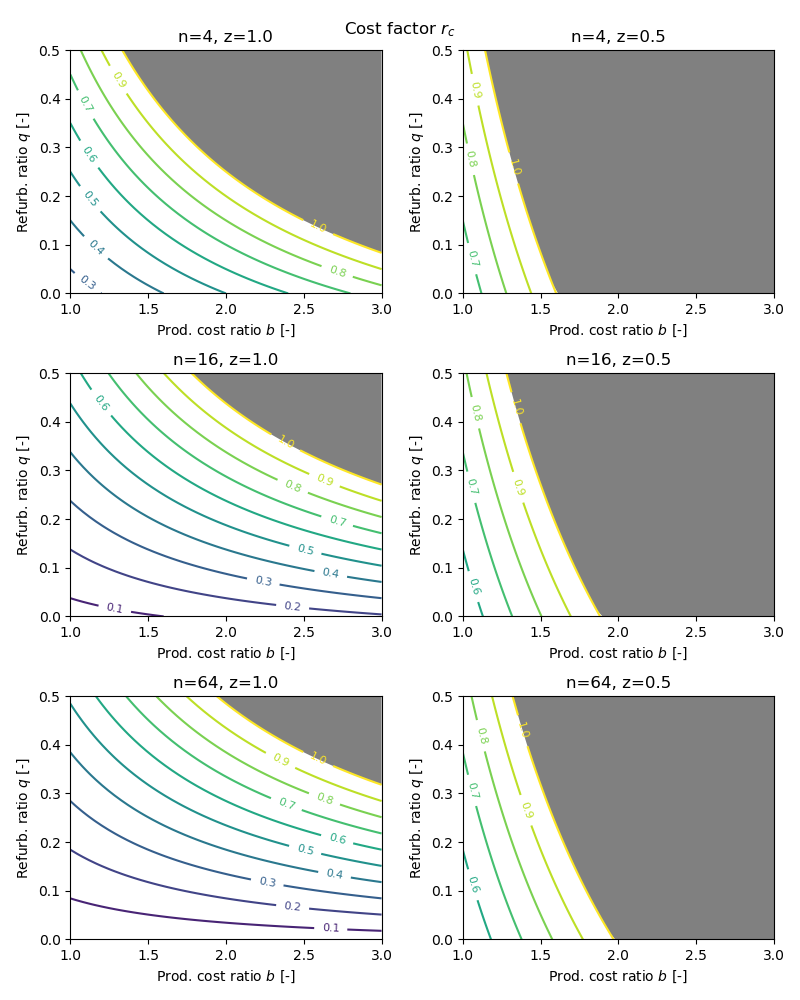
\includegraphics[width=1\textwidth]{../cost_model}
	\label{fig:cost_model}
	\caption{First stage re-use cost factor $r_c$ as a function of the recovery and refurbishment cost ratio $q$ and the production cost ratio $b$. Impractical regimes where re-use would not reduce cost ($r_c>1$) are shaded grey. The plots in the left column correspond to full recovery strategies ($z=1$), and the right to partial recovery ($z=0.5$). The top row corresponds to a conservative reusable component life ($n=4$ flights), the middle to a moderate life ($n=16$) and the bottom to an optimistic life ($n=64$).}
\end{figure}

To facilitate later comparisons of full vs partial recovery strategies, I compute their cost ratios in two scenarios: one making optimistic assumptions about the other variables in the reuse cost model, and one making more moderate assumptions. Table \ref{tab:cost_scenarios} shows that we can reasonably expect the cost factor to be between $0.05$ and $0.52$ for full recovery, and $0.78$ or more for partial recovery. The moderate-assumption case agrees with other assessments that a fully reusable first stage can reduce launch costs "by a factor of 2 to 3" \cite{Hampsten2010}.

\begin{table}
\caption{\label{tab:cost_scenarios} Cost factor $r_c$ in hypothetical reuse scenarios}
\centering
\begin{tabular}{lcc}
\hline
& Optimistic & Moderate \\
& $q=0.02, b=1.5, n=64$ & $q=0.20, b=2.0, n=16$ \\
\hline
Full recovery $z=1$ & 0.05 & 0.53 \\
Partial recovery $z=0.5$ & 0.78 & 1.3 \\
\hline
\end{tabular}
\end{table}


\section{Cost \& Performance Tradeoffs/Comparison}
TODO
The trade a launch operator is willing to make depends on many complicated, context specific factors (cost structure, payload discretization, etc.). Therefore, it is not possible to specify a single strategy as being `best'. Rather, this section seeks to identify the set of Pareto-optimal strategies, each of which offers the greatest payload for a certain level of cost reduction.

Pareto set of best strategies.


\bibliography{first_stage_recovery}

\end{document}